\documentclass[a4paper, 12pt, twoside]{article}
\usepackage[T2A,T1]{fontenc}
\usepackage[utf8]{inputenc}
\usepackage[english, russian]{babel}
\usepackage{graphicx}
\usepackage[hcentering, bindingoffset = 10mm, right = 15 mm, left = 15 mm, top=20mm, bottom = 20 mm]{geometry}
\usepackage{multirow}
\usepackage{lipsum}
\usepackage{amsmath, amstext}
\usepackage{siunitx}
\usepackage{subcaption}
\usepackage{wrapfig}
\usepackage{adjustbox}
\usepackage{enumerate, indentfirst, float}
\usepackage{capt-of, svg}
\usepackage{ctable}
\newcommand*{\hm}[1]{#1\nobreak\discretionary{} 
	{\hbox{$\mathsurround=0pt #1$}}{}}
\usepackage{cmap} % Улучшенный поиск русских слов в полученном pdf-файле

\usepackage{pscyr} % Нормальные шрифты
\usepackage[normalem]{ulem} % для подчёркиваний uline
\ULdepth = 0.16em

\usepackage{fancyhdr} %Колонтикулы
\pagestyle{fancy}
\lhead{
\includegraphics[width = 10 mm]{logo.jpg} Лабораторная работа № 3.3.3}
\rhead{\textit{\today}}

\newenvironment{bottompar}{\par\vspace*{\fill}}{\clearpage}
 
\begin{document}
\begin{titlepage}

\newcommand{\HRule}{\rule{\linewidth}{0.7mm}} % Defines a new command for the horizontal lines, change thickness here

\center % Center everything on the page
 
%----------------------------------------------------------------------------------------
%	HEADING SECTIONS
%----------------------------------------------------------------------------------------

\textsc{\LARGE Московский Физико-Технический Институт}\\[1,5cm] % Name of your university/college
\textsc{\Large Кафедра общей физики}\\[0.5cm] % Major heading such as course name
\textsc{\large Лабораторная работа \textnumero  3.3.3}\\[0.5cm] % Minor heading such as course title

%----------------------------------------------------------------------------------------
%	TITLE SECTION
%----------------------------------------------------------------------------------------

\HRule
\\[0.4cm]
{ \huge \bfseries Опыт Милликена.}
\\[0.2cm] % Title of your document
\HRule
\\[1.5cm]


 
%----------------------------------------------------------------------------------------
%	AUTHOR SECTION
%----------------------------------------------------------------------------------------

\begin{minipage}{0.4\textwidth}
	\begin{flushleft} \large
		\textbf{Автор:}\\
		Глеб Уваркин \\
		615 группа
	\end{flushleft}
\end{minipage}
~
\begin{minipage}{0.4\textwidth}
	\begin{flushright} \large
		\textbf {Преподаватель:} \\
		Андрей Александрович Заболотных % Supervisor's Name
	\end{flushright}
\end{minipage}

\begin{bottompar}
	\begin{center}
		
\includegraphics[width = 80 mm]{logo.jpg}
	\end{center}
	{\large \today}

\end{bottompar}
\vfill % Fill the rest of the page with whitespace

\end{titlepage}

{\Large \uline { \textbf  {Цель работы:}}}

\vspace{2mm}
Измерение элементарного заряда методом масляных капель.
\vspace{\baselineskip}

{\Large \uline { \textbf  {В работе используются:}}}

\vspace{2mm}

Плоский конденсатор в защитном кожухе, осветитель, измерительный микроскоп, выпрямитель, электростатический вольтметр, переключатель напряжения, пульверизатор с маслом, секундомер.

\section{Теоретические сведения.}


Идея опыта очень проста. Если элементарный заряд действительно существует, то заряд $q$ любого тела может принимать только дискретную последовательность значений:
\begin{equation}
\label{f1}
q = 0, \pm e, \pm 2e, \pm 3e, ~ \ldots \pm ne,~ \ldots ,
\end{equation}
где $e$ - заряд электрона. В предлагаемом опыте измеряется заряд небольших капелек масла, несущих всего несколько электронных зарядов. Сравнивая между собой заряды капель, можно убедиться, что все они кратны одному и тому же числу, которое и равно, очевидно, заряду электрона.

Для измерения заряда капель можно исследовать их движение в вертикальном электрическом поле плоского конденсатора.

Движение заряженной капли в электрическом поле зависит как от электрических сил, так и от веча капли. Вес капли может быть определён по скорости её падения в отсутствии поля.

Рассмотрим свободное падение капли. Уравнение её движения при падении имеет вид 
\begin{equation}
\label{f2}
m\dfrac{dv}{dt} = P - F_{\text{тр}},
\end{equation}
где $P$ - вес капли, $v$ - её скорость, а $F_{\text{тр}}$ - сила трения капли о воздух. Сила трения сферической капли определяется формулой Стокса:

\begin{equation}
\label{f3}
F_{\text{тр}} = 6\pi \eta rv = kv,
\end{equation}
где $r$ - радиус капли, $\eta$ - коэффициент внутреннего трения воздуха, $k = 6\pi \eta r$.

Подставляя (\ref{f3}) в (\ref{f2}), найдём
\begin{equation}
\label{f4}
m\dfrac{dv}{dt} = mg - kv.
\end{equation}

Как нетрудно убедиться, решение этого уравнения имеет вид
\begin{equation}
\label{f5}
v = \dfrac{mg}{k}\left(1 - e^{kt/m} \right )
\end{equation}

Установившееся значение скорости равно
\begin{equation}
\label{f6}
v_{\text{уст}} = \dfrac{mg}{k} = \dfrac{\frac{4}{3}\pi r^{3}g}{6\pi \eta r} = \dfrac{2}{9} \dfrac{\rho}{\eta}gr^{2},
\end{equation}

здесь $\rho$ - плотность масла. Заметим, что (\ref{f6}) может быть немедленно получено из (\ref{f4}), если положить $dv/dt = 0$.

Как следует из (\ref{f5}), установление скорости происходит с постоянной времени 
\begin{equation}
\label{f7}
\tau = \dfrac{m}{k} = \dfrac{2}{9} \dfrac{\rho}{\eta}r^{2}.
\end{equation}

Время установления скорости, таким образом, быстро падает с уменьшением радиуса капли r. Для мелких капель оно столь мало, что движение капли всегда можно считать равномерным. Выражение (\ref{f6}) в этом случае определяет радиус капли через скорость её падения. Обозначая через $h$ путь, пройденный каплей за время $t_0$, найдём
\begin{equation}
\label{f8}
r = \sqrt{\dfrac{9\eta h}{2\rho g t_{0}}}.
\end{equation}

Рассмотрим теперь движение капли в присутствии электрического поля. Напряжённость поля $E$ в конденсаторе равна
\begin{equation}
\label{f9}
E = \dfrac{V}{l},
\end{equation}
где $l$ - расстояние между пластинами, а $V$ - разность потенциалов между ними, измеряемая с помощью вольтметра.

Нас будет интересовать случай, когда поле заставляет каплю подниматься. Уравнение движения при этом имеет вид
\begin{equation}
\label{f10}
m\dfrac{dv}{dt} = \dfrac{qV}{l} - mg - kv,
\end{equation}
где $q$ - заряд капли. Прибавление постоянного члена не изменяет постоянной времени $\tau$, с коротой устанавливается скорость капли. Для определения установившейся скорости мы можем снова положить левую часть (\ref{f10}) равной нулю.

Измерим время $t$ подъёма капли на начальную высоту. Используя равенства (\ref{f4}), (\ref{f8}) и (\ref{f10}), найдём, что заряд капли равен
\begin{equation}
\label{f11}
q = 9\pi \sqrt{\dfrac{2\eta^{3}h^{3}}{\text{g}p}}\cdot \dfrac{l(t_{0} + t)}{V t_{0}^{3/2}t}.
\end{equation}
\newpage
\section{Экспериментальная установка.}

\begin{figure}[H]
	\centering
	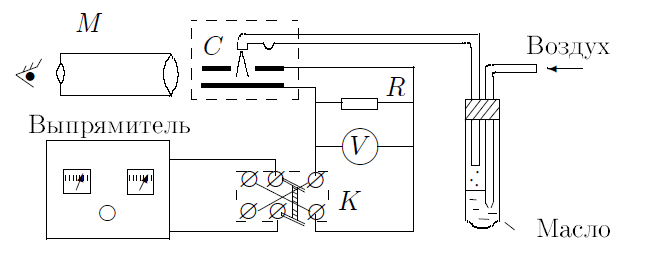
\includegraphics[width = 0.6 \textwidth]{ust}
	\caption{Схема экспериментальной установки для измерения заряда электрона.}
	\label{ust}
\end{figure}

Схема установки представлена на рис. \ref{ust}. Масло разбрызгивается пульверизатором. капли масла попадают в конденсатор $C$ через небольшое отверстие в верхней пластине. При этом часть из них вследствие трения о воздух приобретает случайный по абсолютной величине и знаку электрический заряд.

Напряжение на пластины подаётся с регулируемого выпрямителя и измеряется вольтметром $V$. Ключ $\CYRK$ позволяет менять направление поля в конденсаторе, чтобы можно было работать как с отрицательно, так и с положительно заряженными каплями. При размыкании ключа $\CYRK$ конденсатор разряжается через дополнительное сопротивление  $R \approx 10\text{МОм.}$

Время отсчитывается по секундомеру.

Естественно, что слабые электрические силы, действующие на каплю, несущую всего один или несколько электронных зарядов, способны существенно изменить её движение в том случае, если сама она очень мала. Опыт производится поэтому с мелкими каплями, наблюдение за которыми возможно только с помощью микроскопа.

В фокальной плоскости окуляра измерительного микроскопа $\CYRM$ виден ряд горизонтальных линий, расстояние между которыми было предварительно определено с помощью объектного микрометра. Наблюдая за перемещением капли между нитями, нетрудно определить путь, пройденный каплей. Время $t_0$ свободного падения капли от одной выбранной линии до другой и время $t$ её обратного подъёма, происходящего под действием сил электрического поля, измеряется секундомером.

Из постановки опыта очевидно, что дискретность заряда может быть обнаружена лишь в том случае, если ошибка $\delta q$ в измерении заряда капли существенно меньше абсолютной величины заряда электрона $e$. Допустимая относительная ошибка опыта $\delta q/q$ должна быть поэтому много меньше $e/q = 1/n$, где $n$ - заряд капли, выраженный в числе зарядов электрона. Этому условию тем легче удовлетворить, чем меньше число $n$. В нашем случае трудно определить $q$ с точностью лучше $5\%$. Заряд капли должен поэтому быть существенно меньше 20 зарядов электрона - лучше всего, если он не превосходит пяти электронных зарядов.
\newpage
\section{Обработка результатов.}

Проведём серию измерений для 7 капель, а именно: измерим время их падения под действием силы тяжести на расстояние $h = 1$ мм и время их подъёма под действием электрических сил также на расстояние $h = 1$ мм.

Запишем полученные данные в таблицу \ref{t1}. Для всех капель рассчитаем значения $q$, а также $\sigma_q$ по формуле:
$$\sigma_q = q\sqrt{\dfrac{\sigma_V^2}{V^2} + \dfrac{\sigma_t^2 t_0^2}{t^2(t_0+t)^2} + \dfrac{\sigma_{t_0}^2}{4t_0^2} \left(\dfrac{3t+t_0}{t+t_0}\right)^2},$$

где $\sigma_V = 10$ В, $\sigma_t=\sigma_{t_0}\simeq 0.2$ с.

\begin{table}[H]
	\centering
	\caption{Полученные данные.}
	\label{t1}
	\resizebox{\textwidth}{!}{
	\begin{tabular}{c|ccccc|ccccc|ccccc}
		\toprule
		Капля № & \multicolumn{5}{c|}{1}        & \multicolumn{5}{c|}{2}         & \multicolumn{5}{c}{3}         \\ \midrule
		$V,$ В     & \multicolumn{5}{c|}{1000}        & \multicolumn{5}{c|}{970}         & \multicolumn{5}{c}{800}         \\ \midrule
		$t_0,$ сек & 21.9 & 22.3 & 23.7 & 21.7 & 22.4 & 21.3 & 21.5 & 21.3 & 21.2 & 20.5 & 21.8 & 20.5 & 20.4 & 20.9 & 20.7 \\
		$t,$ сек   & 34.7 & 33.7 & 38.7 & 35.7 & 35.1 & 42.2 & 41.4 & 40.3 & 40.7 & 40.7 & 74.2 & 72.3 & 77.1 & 74.4 & 75.2 \\ \midrule
		$q\cdot 10^{-19},$ Кл    & 1.22  &  1.21 & 1.07  & 1.22   & 1.18  & 1.21  & 1.20  & 1.23 & 1.23     & 1.28     &  1.22    &  1.32    & 1.31     & 1.28     & 1.29 \\ 
		$\sigma_q\cdot 10^{-19},$ Кл &0.02&0.02&0.01&0.02&0.02&0.02&0.02&0.02&0.02&0.02&0.02&0.02&0.02&0.02&0.02 \\ \bottomrule
		  
	\end{tabular}
}
\end{table}

\begin{table}[H]
	\centering
	\resizebox{\textwidth}{!}{
	\begin{tabular}{c|ccccc|ccccc|ccccc} \toprule
			Капля № & \multicolumn{5}{c|}{4}        & \multicolumn{5}{c|}{5}         & \multicolumn{5}{c}{6}         \\ \midrule
		$V,$ В     & \multicolumn{5}{c|}{980}         & \multicolumn{5}{c|}{1000}        & \multicolumn{5}{c}{860}          \\ \midrule
		$t_0,$ сек & 18.4 & 18.5 & 17.8 & 18.4 & 18.3 & 16.5 & 16.1 & 15.8 & 15.4 & 16.3 & 9.2  & 9.2  & 9    & 9.4  & 9.3  \\
		$t,$ сек   & 68.3 & 66.1 & 69.8 & 68.2 & 71.7 & 14.4 & 15.0 & 15.4 & 14.9 & 15.6 & 66.2 & 71.4 & 72.4 & 75.6 & 76.2 \\ \midrule
		$q\cdot 10^{-19},$ Кл    & 1.25     & 1.25     & 1.30     & 1.26     & 1.25     & 2.45     & 2.45     & 2.47     & 2.57     &  2.38    & 3.63     & 3.60     & 3.70     & 3.47     & 3.52    \\ 
		$\sigma_q\cdot 10^{-19},$ Кл &0.02&0.02&0.01&0.02&0.02&0.04&0.04&0.04&0.05&0.04&0.12&0.12&0.12&0.12&0.12 \\ \bottomrule
	\end{tabular}
}
\end{table}

\begin{table}[H]
	\centering
	\resizebox{0.42\textwidth}{!}{
	\begin{tabular}{c|ccccc} \toprule
			Капля № & \multicolumn{5}{c}{7}  \\ \midrule
		$V,$ В     & \multicolumn{5}{c}{1000}         \\ \midrule
		$t_0,$ сек & 10.3 & 10.3 & 10.1 & 10.2 & 10.2 \\
		$t,$ сек   & 20.4 & 20.4 & 20.1 & 20.9 & 20.5 \\ \midrule
		$q\cdot 10^{-19},$ Кл    & 3.48 & 3.48     &  3.58    & 3.49     & 3.52 \\ 
		$\sigma_q\cdot 10^{-19},$ Кл &0.09&0.09&0.09&0.09&0.09 \\ \bottomrule  
	\end{tabular}
}
\end{table}

Усредним значения $q$ для каждой капли, занесём данные в таблицу \ref{t2}.

\begin{table}[H]
	\centering
	\caption{Средние значения заряда капли.}
	\label{t2}
		\begin{tabular}{c|ccccccc} \toprule
			Капля № & 1&2&3&4&5&6&7  \\ \midrule
			$q_{\text{ср}}\cdot 10^{-19},$ Кл    & 1.18	 & 1.23     &  1.28    & 1.26     & 2.46 & 3.58& 3.51 \\ 
			$\sigma_q\cdot 10^{-19},$ Кл &0.02&0.02&0.02&0.02&0.05&0.12&0.09 \\
			$\varepsilon_q, \%$ &2&2&2&2&2&3&3 \\ 
			\bottomrule  
		\end{tabular}
\end{table}

\begin{figure}[H]
	\centering
	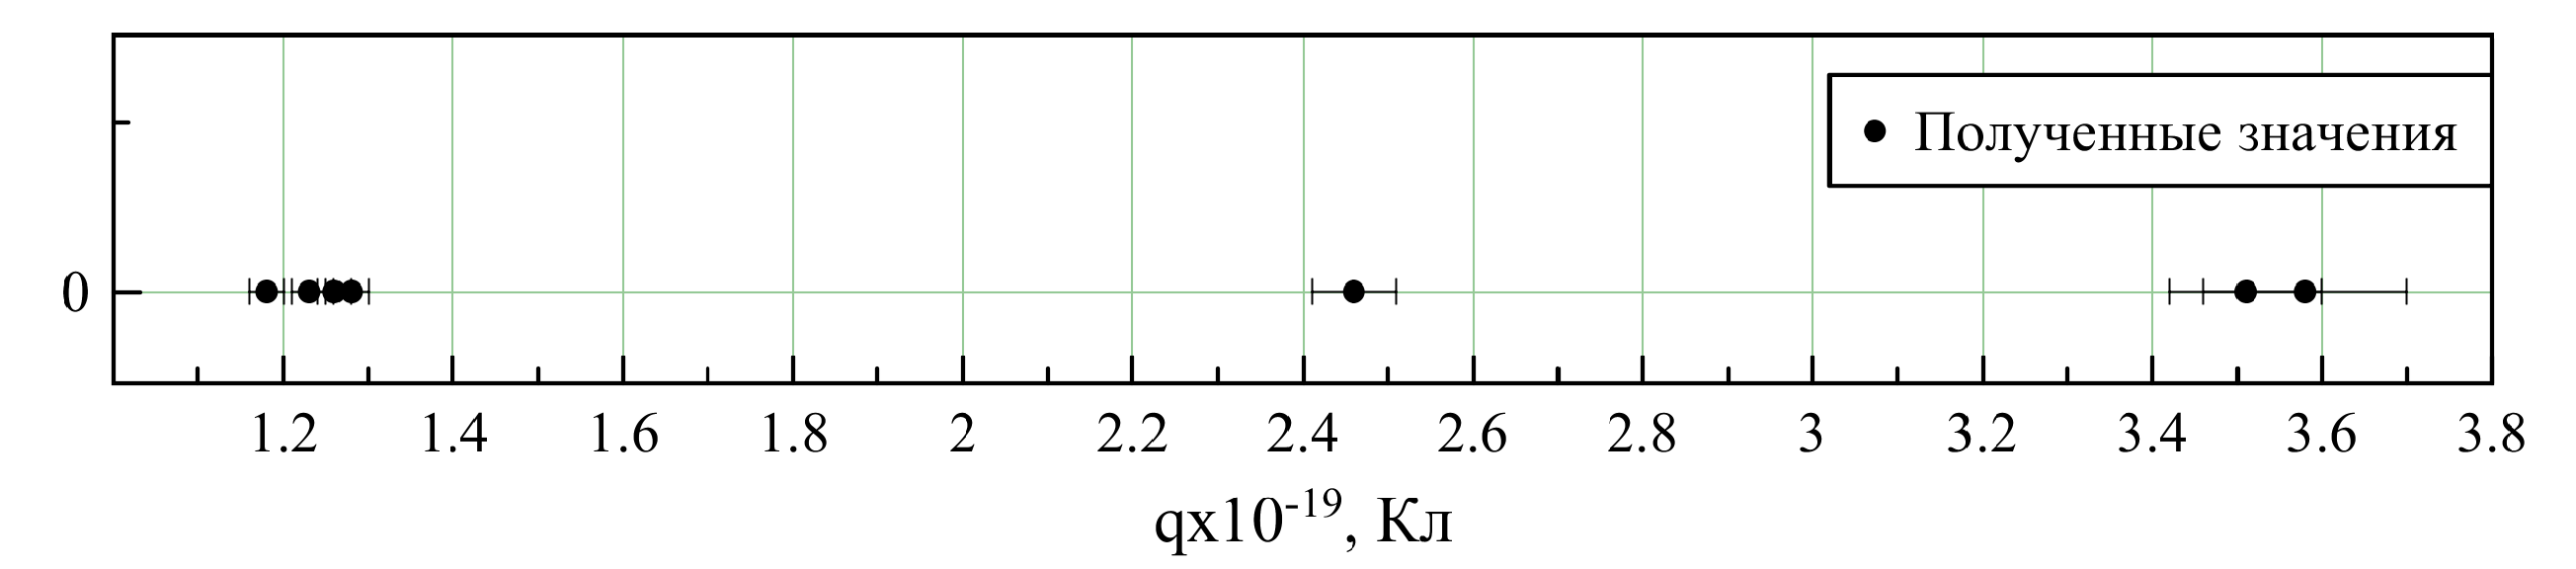
\includegraphics[width =  \textwidth]{graph}
	\caption{Полученные значения $q$.}
	\label{ust}
\end{figure}

Получаем, что наибольший общий делитель для всех измеренных капель равен
\begin{equation*}
\fbox{\text{$
|e| \simeq (1.25 \pm 0.12) \cdot 10^{-19} \text{Кл} \simeq (3.75 \pm 0.36) \cdot 10^{-10}\text{ед. СГСЭ}~(\varepsilon \simeq 10 \%)$}} 
\end{equation*}
\\

"Подвесим" одну из капель в электрическом поле. Определим соответствующее напряжение, отключим его и измерим время падения капли на расстояние $h = 0.75\text{мм}$. Поменяв полярность напряжения, вернём каплю на прежнее место и снова подвесим её. Снова запишем напряжение. Повторим процедуру для данной капли несколько раз, запишем результаты в таблицу \ref{table}, оценим из этого опыта заряд капли по формуле (\ref{f11}), полагая время подъема $t = \infty$. По разбросу результатов ($\Delta V ~\text{и}~ \Delta{t}$) оценим точность измерения заряда этой капли.

$$(11) \underset{t\longrightarrow \infty}{\Longrightarrow} q = 9\pi \sqrt{\dfrac{2\eta^{3}h^{3}}{\text{g}p}}\cdot \dfrac{l}{Vt_0^{3/2}}. $$

\begin{table}[H]
	\centering
	\caption{Измерение капли.}
	\label{table}
	\begin{tabular}{c|ccccc}
		\toprule
		$V,$ В    & 680 & 680 & 680 & 680 & 680 \\
		$t_0, $ с & 7.6 & 7.6 & 7.4 & 7.3 & 7.6\\ \midrule
		$q\cdot 10^{-19},$ Кл &3.49&3.49&3.63&3.70&3.49 \\
		 \bottomrule
	\end{tabular}
\end{table}
\begin{equation*}
\fbox{\text{$
q_{\text{ср}} = (3.56 \pm 0.09) \cdot 10^{-19}~\text{Кл}~(\varepsilon \simeq 3 \%)$}}
\end{equation*}
\\

Оценим максимальный путь релаксации $s$ в условиях эксперимента:
$$s = v_{\text{уст}}\tau = \dfrac{1}{\text{g}}\left (\dfrac{h}{t_0}\right ) ^2 = \dfrac{1}{9.8}\left ( \dfrac{10^{-3}}{9}\right ) ^2 \simeq 1.26~\text{нм}$$ 

\section{Вывод.}

Полученное значение элементарного заряда отличается от табличного на $30\%$. Причиной этому могли послужить несколько факторов:
\begin{itemize}
	\item систематическая ошибка установки(все полученные заряды не кратны табличному значению элементарного заряда)
	\item ошибка наблюдающего при выборе капли (от правильности выбора капли зависит  точность измерения)
	\item засвеченность окуляра, которая не позволила с высокой точностью определить время прохождения нужного расстояние каплей
	\item человеческий фактор
\end{itemize}





\end{document}